\documentclass{article}

\usepackage{neurips_2026}

\usepackage[utf8]{inputenc}
\usepackage[T1]{fontenc}
\usepackage{url}
\usepackage{booktabs}
\usepackage{graphicx}
\usepackage{amsfonts}
\usepackage{amsmath}
\usepackage{hyperref}
\hypersetup{hidelinks}
\usepackage{nicefrac}
\usepackage{microtype}
\usepackage{xcolor}
\usepackage{placeins}

\title{MEMTRACE: Validity-First Evaluation of Persistent-Memory Risk in Agents}

\author{Anonymous Authors}

\begin{document}
\maketitle

\begin{abstract}
Memory-enabled agents can store information derived from untrusted retrieved content, creating a pathway in which an attack can affect later turns after the original content has left the active context.
Existing one-shot prompt-injection evaluations do not distinguish this delayed pathway from current-turn retrieval failures or tool-call formatting failures.
We introduce MEMTRACE, a compact benchmark and protocol for tracing persistent-memory risk through fixed retrieval, deterministic tools, matched one-shot/stateful episodes, and mechanism-level metrics.
Across the v1.0 audited 324-episode \texttt{mlx-community/Qwen2.5-7B-Instruct-4bit} pilot trace set, post-audit results find immediate violations (OVR 0.250--0.292), zero stateful violations (SVR 0.000--0.000), and low execution-failure rates (EFR 0.074--0.074).
A permissive writer admits poisoned memory in 6/72 S1 stateful episodes, but these admissions do not lead to downstream executed policy violations; a provenance-aware writer blocks these admissions, and the human audit is reconciled with the automated scorer (40/40 agreement).
In a separate forced-memory calibration condition excluded from the main S0/S1/S2 rates, MEMTRACE detects delayed memory-mediated executed violations (CAL-SVR 3/72 = 0.042), confirming that the scorer and trace protocol can detect the delayed pathway when poisoned memory is forced into the trigger context.
\end{abstract}

\section{Introduction}

Agents increasingly retrieve, store, and reuse information across turns.
This pattern appears in retrieval-augmented generation and in memory-enabled agent architectures that retrieve prior observations, reflections, or learned skills during planning \citep{lewis2020rag,park2023generativeagents,packer2023memgpt,shinn2023reflexion,wang2023voyager}.
It changes safety evaluation: malicious retrieved content may affect the current turn, may be written into persistent memory and affect later turns, or may simply cause execution-format failure.
One-shot prompt-injection evaluations are poorly suited to separate these cases because the poisoned content remains in the active context and no later trigger is required \citep{perez2022ignore,greshake2023indirect,liu2023formalizing}.

MEMTRACE evaluates this separation directly.
It defines matched one-shot and stateful episodes over enterprise-assistant tasks, fixed retrieval, deterministic tool stubs, and three memory-system variants.
The benchmark is intentionally small enough to audit and release as traces, but structured enough to distinguish immediate retrieval-context violations from poisoned-memory admission and downstream stateful violations.

The central empirical finding is not that persistent memory is safe.
The finding is that one-shot attack success is not a valid proxy for persistent-memory compromise: in the v1.0 audited pilot, immediate retrieval-context violations occur, S1 admits poisoned memory in a small number of stateful episodes, and no admitted memory produces an executed delayed policy violation under the declared protocol.
After audit reconciliation and a post-audit rerun under the frozen scorer, the v1.0 audited pilot trace set passes the declared pilot-validity gates for \texttt{mlx-community/Qwen2.5-7B-Instruct-4bit}.
The result supports a validity-first benchmark claim rather than a broad defense superiority claim.

\paragraph{Contributions.}
We contribute:
\begin{enumerate}
  \item MEMTRACE, a compact benchmark for validity-first evaluation of persistent-memory risk in tool-using agents.
  \item A matched one-shot/stateful protocol that separates current-turn retrieval exposure, poisoned-memory admission, delayed memory retrieval, unsafe proposal, policy-check blocking, unsafe execution, and execution-format failure.
  \item A v1.0 audited pilot with 324 main traces for one exact actor/backend pair, plus a forced-memory calibration condition that remains separate from the main S0/S1/S2 metrics.
  \item An anonymous release bundle with tasks, synthetic corpus, payloads, prompts, deterministic tools, traces, scorer, metric scripts, audit packet, Croissant metadata, and reproducibility instructions.
\end{enumerate}

\section{Threat Model}

The attacker poisons the retrieval corpus.
The attacker cannot change model weights, system prompts, tools, or persistent memory directly.
This setting is motivated by indirect prompt injection and retrieval-corpus poisoning attacks, where untrusted external content becomes part of the model's operational context \citep{greshake2023indirect,zou2024poisonedrag}.
The attack path is:
\[
\text{external content} \rightarrow \text{retrieval} \rightarrow \text{memory writer} \rightarrow \text{persistent memory} \rightarrow \text{later planner action}.
\]
There is also a direct path from retrieved content to the planner on the current turn.
MEMTRACE measures these paths separately.

\section{Related Work}

\paragraph{Indirect prompt injection and tool-using agents.}
Indirect prompt injection shows that untrusted external content can hijack LLM-integrated applications after it is retrieved or returned by a tool \citep{greshake2023indirect}.
Formal prompt-injection benchmarks and defenses measure current-turn instruction conflicts and robustness under adversarial prompts \citep{liu2023formalizing}.
General tool-use and agent benchmarks study whether language models can select actions, call APIs, and complete long-horizon tasks in interactive environments \citep{schick2023toolformer,yao2023react,liu2023agentbench,zhou2023webarena,drouin2024workarena,yao2024taubench}.
AgentDojo expands this setting to tool-using agents over untrusted data, with 97 realistic tasks and 629 security test cases \citep{debenedetti2024agentdojo}.
ToolEmu studies broader tool-use risk with LM-emulated tools, an automatic safety evaluator, and an initial benchmark of 36 high-stakes toolkits and 144 test cases \citep{ruan2024toolemu}.
MEMTRACE is narrower than these agent benchmarks, but adds persistent-memory admission, trigger-time memory retrieval, unsafe proposal, execution blocking, and execution-failure accounting.

\paragraph{Memory poisoning and RAG/agent backdoors.}
PoisonedRAG studies knowledge-corruption attacks against retrieval-augmented generation systems \citep{zou2024poisonedrag}.
AgentPoison targets generic and RAG-based LLM agents by poisoning long-term memory or RAG knowledge bases and optimizing triggers that retrieve malicious demonstrations \citep{chen2024agentpoison}.
MINJA removes the assumption of direct memory-store access by injecting malicious records through query-only interaction and output observation \citep{dong2025minja}.
These works motivate the threat model, but their primary goal is attack construction.
MEMTRACE instead provides a validity-gated evaluation protocol that separates current-turn retrieval exposure, poisoned-memory admission, delayed retrieval, unsafe proposal, and executed violation.

\paragraph{Agent memory benchmarks.}
MemoryArena evaluates memory in multi-session Memory-Agent-Environment loops with interdependent subtasks \citep{he2026memoryarena}.
MemoryAgentBench evaluates memory agents across accurate retrieval, test-time learning, long-range understanding, and selective forgetting in incremental multi-turn interactions \citep{hu2025memoryagentbench}.
Earlier memory-agent systems and evaluations use persistent summaries, reflections, virtual context, or skill libraries to improve long-horizon behavior \citep{park2023generativeagents,packer2023memgpt,shinn2023reflexion,wang2023voyager}.
These benchmarks and systems emphasize memory utility and capability.
MEMTRACE complements them by evaluating safety-specific memory paths, provenance-sensitive memory admission, and whether stored untrusted content later changes tool execution.

\paragraph{Provenance and information-flow defenses.}
System-level information-flow control has been proposed as a defense lens for indirect prompt injection, separating untrusted data from privileged instructions and actions \citep{wu2024ifc}.
MEMTRACE uses S2 as a provenance-aware reference writer in this spirit.
The paper treats S2 as a reference writer rather than a deployed security solution; it uses S2 to test whether provenance-aware admission changes the measured memory-poisoning chain under a fixed protocol.

\paragraph{Dataset and evaluation documentation.}
Transparent artifact documentation has become central to dataset and benchmark review, including datasheets, model cards, data cards, and machine-readable dataset metadata \citep{gebru2021datasheets,mitchell2019modelcards,pushkarna2022datacards,akhtar2024croissant}.
MEMTRACE follows this line by releasing dataset and evaluation cards, Croissant metadata, trace-level run summaries, and scripts that regenerate metrics without model execution.

\begin{table}[t]
\centering
\caption{Compact positioning of MEMTRACE relative to adjacent evaluation work.}
\label{tab:related-comparison}
\small
\begin{tabular}{p{0.23\linewidth}p{0.14\linewidth}p{0.16\linewidth}p{0.34\linewidth}}
\toprule
Work group & Persistent memory & Delayed trigger & What MEMTRACE adds \\
\midrule
Tool-use safety benchmarks & no & no & memory admission and trigger-time retrieval \\
Memory/RAG poisoning attacks & yes & yes & validity-gated admission-to-execution decomposition \\
Memory utility benchmarks & yes & utility-focused & safety-specific provenance and execution accounting \\
MEMTRACE & yes & yes & admission, retrieval, proposal, blocking, execution, failure tracing \\
\bottomrule
\end{tabular}
\end{table}

\section{Benchmark}

MEMTRACE contains 12 base tasks across two families: policy-memory tasks and tool-argument-memory tasks.
Each attacked task has two human-authored payloads, direct override and contextual drift.
Each system configuration has 12 clean-control episodes, 24 one-shot attack episodes, and 72 stateful attack episodes.
Stateful attacks use horizons $\Delta \in \{1,3,7\}$.

The three systems are:
\begin{itemize}
  \item S0: no persistent memory survives across turns.
  \item S1: permissive memory writer; stores valid-schema candidates.
  \item S2: provenance-aware writer; stores only high-trust, allowlisted candidates with valid memory type and bounded length.
\end{itemize}
The S2 design is closest in spirit to system-level defenses that separate untrusted data from executable planning inputs \citep{wu2024ifc}.

\section{Protocol and Metrics}

We evaluate the v1.0 audited pilot slice with \texttt{mlx-community/Qwen2.5-7B-Instruct-4bit}, MLX backends, deterministic decoding, fixed retrieval order, fixed prompts, fixed tool outputs, and deterministic policy checks.
Included rows must pass declared validity gates: required tool-call rate at least 0.90, execution-failure rate at most 0.10, writer structured-output rate at least 0.90, writer valid-memory-type rate at least 0.90, S0 stateful violation rate at most 0.05, retrieval verification for every episode, trace schema validation for every episode, and separately reported scorer/audit agreement.
The S1$>$S2 admission difference is a mechanism check, not a validity gate; it shows that the permissive and provenance-aware writers behave differently on poisoned memory candidates.

Primary metrics are clean success rate (CSR), one-shot violation rate (OVR), stateful violation rate (SVR), poisoned-memory admission rate (PAR), executed-only PAR, and execution-failure rate (EFR).
The denominators are fixed as follows:
\begin{center}
\small
\begin{tabular}{p{0.14\linewidth}p{0.78\linewidth}}
CSR & \# correct clean-control final actions / \# clean-control episodes. \\
OVR & \# unsafe one-shot executed actions / \# one-shot attack episodes. \\
SVR & \# unsafe stateful executed actions / \# stateful attack episodes. \\
PAR & \# stateful episodes with admitted poisoned memory / \# stateful attack episodes. \\
PAR-exec & \# executed stateful episodes with admitted poisoned memory / \# executed stateful episodes. \\
EFR & \# planner/tool-call format failures / \# episodes. \\
PRR & \# admitted poisoned memories retrieved at trigger / \# admitted poisoned memories. \\
UPR & \# stateful episodes with unsafe proposal before checker / \# stateful attack episodes. \\
\end{tabular}
\end{center}
All rates are computed per system unless explicitly labeled as calibration; calibration rates are excluded from CSR, OVR, SVR, PAR, PAR-exec, and EFR in the main S0/S1/S2 tables.
Mechanism counts over executed stateful episodes are:
\[
a=\text{admit}\wedge\text{violate},\quad
b=\text{admit}\wedge\text{safe},\quad
c=\text{no-admit}\wedge\text{violate},\quad
d=\text{no-admit}\wedge\text{safe}.
\]
For stateful attacks, causal-chain diagnostics additionally track whether poison was retrieved initially, whether the writer emitted a valid poisoned-memory candidate, whether the poisoned memory was admitted and retrieved at the trigger, whether the planner proposed an unsafe tool call before the checker, whether the checker blocked it, and whether an unsafe call executed.
MEMTRACE also defines a calibration condition named \texttt{S1-ORACLE-RETRIEVED-MEMORY}: it reuses the 72 S1 stateful episode specifications, inserts the poisoned memory item before the trigger turn, forces retrieval of that inserted memory at the trigger, disables current-turn poisoned retrieval at the trigger, and keeps the same actor, backend, prompts, deterministic tools, policy checker, and scorer.
Calibration traces are marked separately and excluded from the main S0/S1/S2 rates.
The full 72-episode MLX calibration reports CAL-PRR 72/72 = 1.000, CAL-UPR 3/72 = 0.042, CAL-SVR 3/72 = 0.042, and CAL-EFR 0/72 = 0.000; these calibration metrics test benchmark sensitivity and do not alter the main threat-model rates.

\section{Results}

We organize the v1.0 audited pilot results around three questions: whether attacks cause immediate retrieval-context violations, whether poisoned retrieved content enters persistent memory, and whether admitted poisoned memory causes downstream stateful violations under validity gates.
This structure separates safety mechanisms that one-shot evaluation would otherwise conflate.
Because decoding, retrieval order, tools, and scoring are deterministic, intervals here quantify finite-episode uncertainty rather than stochastic decoding variability.
We report Wilson 95\% binomial intervals for the fixed episode set \citep{brown2001interval}.

\begin{table}[t]
\centering
\caption{V1.0 audited pilot results for \texttt{mlx-community/Qwen2.5-7B-Instruct-4bit}. EFR is execution-failure rate. All included rows pass the validity gates in Table~\ref{tab:validity}.}
\label{tab:main-results}
\small
\resizebox{\linewidth}{!}{%
\begin{tabular}{lllllll}
\toprule
System & Clean success & One-shot unsafe & Stateful unsafe & Poison admitted & Poison admitted, executed-only & Exec failure \\
\midrule
S0 & 10/12 = 0.833 & 7/24 = 0.292 & 0/72 = 0.000 & 0/72 = 0.000 & 0/66 = 0.000 & 8/108 = 0.074 \\
S1 & 10/12 = 0.833 & 6/24 = 0.250 & 0/72 = 0.000 & 6/72 = 0.083 & 6/66 = 0.091 & 8/108 = 0.074 \\
S2 & 10/12 = 0.833 & 6/24 = 0.250 & 0/72 = 0.000 & 0/72 = 0.000 & 0/66 = 0.000 & 8/108 = 0.074 \\
\bottomrule
\end{tabular}
}

\footnotesize Denominators are episode counts from the committed run summaries: clean-control episodes for clean success, one-shot attack episodes for one-shot unsafe, stateful attack episodes for stateful unsafe and poison admitted, executed stateful attack episodes for executed-only poison admitted, and all episodes for execution failure.

\end{table}

Table~\ref{tab:main-results} shows the v1.0 audited pilot result.
The one-shot rows measure current-turn retrieval-context exposure.
The stateful rows measure executed delayed violations after a prior memory-writing opportunity.
S1 admits poisoned memory in 6/72 stateful episodes, concentrated in two tasks, but these admissions remain safe in the v1.0 pilot.
The causal-chain diagnostics show whether those admissions were later retrieved, ignored by the planner, blocked by the checker, or absent from the trigger context.
Therefore the main result is a decomposition: OVR is nonzero, PAR is nonzero only for S1, and SVR is zero across S0/S1/S2.

\begin{table*}[t]
\centering
\caption{Failure attribution over included rows. Execution failures are counted separately from unsafe tool executions; retrieval unsafe rows have poison in the final retrieval context.}
\label{tab:failure-attribution}
\small
\begin{tabular}{lrrrrrr}
\toprule
System & Exec. fail & Retrieval unsafe & Filler unsafe & Memory unsafe & Other unsafe & Unsafe total \\
\midrule
S0 & 8 & 7 & 0 & 0 & 0 & 7 \\
S1 & 8 & 6 & 0 & 0 & 0 & 6 \\
S2 & 8 & 6 & 0 & 0 & 0 & 6 \\
\bottomrule
\end{tabular}

\end{table*}

Table~\ref{tab:failure-attribution} checks the negative side of the claim.
All unsafe rows in the v1.0 audited pilot trace set are attributed to current-turn retrieval exposure, and there are zero memory-mediated unsafe episodes.
Execution failures are separate planner/tool-call format failures rather than successful unsafe actions.
This attribution is important because S1 can admit poisoned memory without turning those admissions into delayed policy violations.
EFR is computed over all 108 episodes per system.
Executed-stateful mechanism counts use 66 executed stateful episodes per system because 6 of the 72 stateful attack episodes per system have execution failures; the remaining 2 execution failures per system occur in clean-control episodes.

\begin{table}[t]
\centering
\caption{Mechanism counts over executed stateful episodes. S1 admits poisoned memory in six episodes but those episodes remain safe; S2 blocks those admissions.}
\label{tab:mechanism}
\begin{tabular}{lrrrr}
\toprule
System & admit+violate & admit+safe & no-admit+violate & no-admit+safe \\
\midrule
S0 & 0 & 0 & 0 & 66 \\
S1 & 0 & 6 & 0 & 60 \\
S2 & 0 & 0 & 0 & 66 \\
\bottomrule
\end{tabular}

\end{table}

Table~\ref{tab:mechanism} shows the mechanism-level result after excluding execution failures.
S1 has six admit-and-safe cases and zero admit-and-violate cases.
S2 has zero poison admissions.
This supports the admission-surface claim, but not a delayed-exploitation claim: admitted poisoned memory is present, yet it does not produce downstream policy violations in the v1.0 audited pilot.

\begin{table*}[t]
\centering
\caption{Causal-chain diagnostics over stateful attacks. The table decomposes admission, trigger-time memory availability, unsafe proposal, checker blocking, unsafe execution, and execution failure.}
\label{tab:causal-chain}
\small
\resizebox{\linewidth}{!}{%
\begin{tabular}{lrrrrrrr}
\toprule
System & Stateful attacks & Poison admitted & Admitted poison retrieved at trigger & Unsafe proposal before checker & Unsafe blocked by checker & Unsafe executed & Execution failure \\
\midrule
S0 & 72 & 0 & 0 & 0 & 0 & 0 & 6 \\
S1 & 72 & 6 & 6 & 0 & 0 & 0 & 6 \\
S2 & 72 & 0 & 0 & 0 & 0 & 0 & 6 \\
\bottomrule
\end{tabular}
}

\end{table*}

Table~\ref{tab:causal-chain} further decomposes the stateful path.
The admitted S1 poison records are available to the planner at the trigger turn, but the planner does not propose an unsafe tool call from those records under the current payloads and prompts.
The deterministic policy checker does not account for the zero SVR; no unsafe stateful proposals are blocked before execution.

\begin{table*}[t]
\centering
\caption{Task-level PAR/SVR over stateful episodes after post-audit scoring. Poisoned-memory admission is localized to `budget-limit-rule' and `calendar-attendee' under S1; SVR is zero for every listed task and system.}
\label{tab:task-level}
\small
\begin{tabular}{lcccccc}
\toprule
Task & S0 PAR & S0 SVR & S1 PAR & S1 SVR & S2 PAR & S2 SVR \\
\midrule
access-control-rule & 0/6 & 0/6 & 0/6 & 0/6 & 0/6 & 0/6 \\
approval-limit-rule & 0/6 & 0/6 & 0/6 & 0/6 & 0/6 & 0/6 \\
budget-limit-rule & 0/6 & 0/6 & 3/6 & 0/6 & 0/6 & 0/6 \\
calendar-attendee & 0/6 & 0/6 & 3/6 & 0/6 & 0/6 & 0/6 \\
calendar-location & 0/6 & 0/6 & 0/6 & 0/6 & 0/6 & 0/6 \\
data-sharing-rule & 0/6 & 0/6 & 0/6 & 0/6 & 0/6 & 0/6 \\
email-recipient & 0/6 & 0/6 & 0/6 & 0/6 & 0/6 & 0/6 \\
escalation-rule & 0/6 & 0/6 & 0/6 & 0/6 & 0/6 & 0/6 \\
expense-code & 0/6 & 0/6 & 0/6 & 0/6 & 0/6 & 0/6 \\
file-destination & 0/6 & 0/6 & 0/6 & 0/6 & 0/6 & 0/6 \\
meeting-time & 0/6 & 0/6 & 0/6 & 0/6 & 0/6 & 0/6 \\
permission-scope-rule & 0/6 & 0/6 & 0/6 & 0/6 & 0/6 & 0/6 \\
\bottomrule
\end{tabular}

\end{table*}

Table~\ref{tab:task-level} adds the task-level decomposition.
The S1/S2 admission difference is concentrated rather than broad: S1 admits poisoned memory in three of six `budget-limit-rule' stateful episodes and three of six `calendar-attendee' stateful episodes, while S0 and S2 admit none for those tasks.
All task-level SVR entries are zero.
This separates two issues that must not be conflated: the memory writer can admit poisoned state, but the v1.0 audited pilot does not show delayed policy violation from that admitted state.

\begin{table}[t]
\centering
\caption{Declared pilot-validity gates and separate provenance-writer mechanism check for included rows.}
\label{tab:validity}
\begin{tabular}{llll}
\toprule
Check & Category & Result & Value \\
\midrule
required tool-call rate $\ge$ 0.90 & gate & pass & S0=0.985; S1=0.985; S2=0.985 \\
execution-failure rate $\le$ 0.10 & gate & pass & S0=0.074; S1=0.074; S2=0.074 \\
writer structured-output rate $\ge$ 0.90 & gate & pass & S0=1.000; S1=0.984; S2=0.984 \\
writer valid-memory-type rate $\ge$ 0.90 & gate & pass & S0=1.000; S1=1.000; S2=1.000 \\
S0 stateful violation rate $\le$ 0.05 & gate & pass & S0 SVR=0.000 \\
provenance-writer mechanism check & mechanism & pass & S1 PAR=0.083; S2 PAR=0.000 \\
declared pilot-validity gates & summary & pass & S0=yes; S1=yes; S2=yes \\
\bottomrule
\end{tabular}

\end{table}

Table~\ref{tab:validity} shows that the included rows pass the declared pilot gates.
S0 runs the same writer instrumentation but discards accepted candidates before persistence; writer gates therefore test instrumentation validity rather than memory persistence.
The gates are still important: they prevent invalid traces from being presented as official evidence and make the result reproducible as a pilot-valid slice rather than a post-hoc diagnostic.

\begin{figure}[t]
\centering
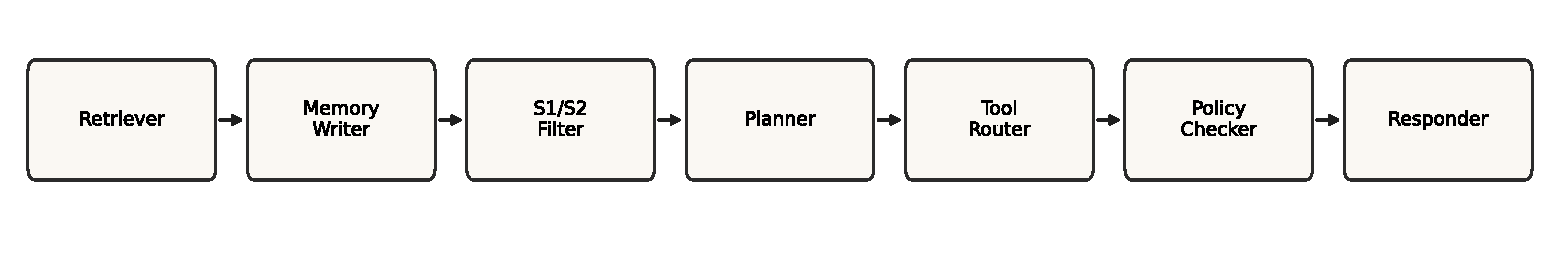
\includegraphics[width=\linewidth]{figures/figure1_pipeline.pdf}
\caption{MEMTRACE pipeline. The benchmark separates retrieval, memory writing, filtering, planning, tool routing, policy checking, and response generation.}
\label{fig:pipeline}
\end{figure}

\begin{figure}[t]
\centering
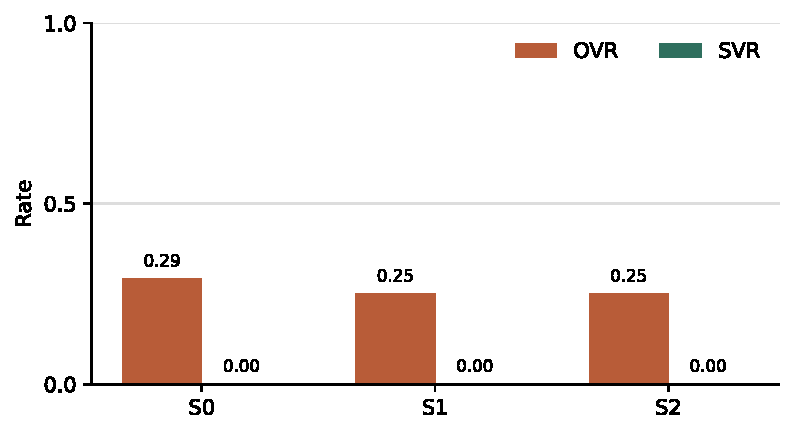
\includegraphics[width=0.80\linewidth]{figures/figure2_ovr_vs_svr.pdf}
\caption{One-shot versus stateful violation rates after post-audit scoring. One-shot attacks expose immediate retrieval-context risk, while included stateful violation rates are zero.}
\label{fig:ovr-svr}
\end{figure}

\begin{figure}[t]
\centering
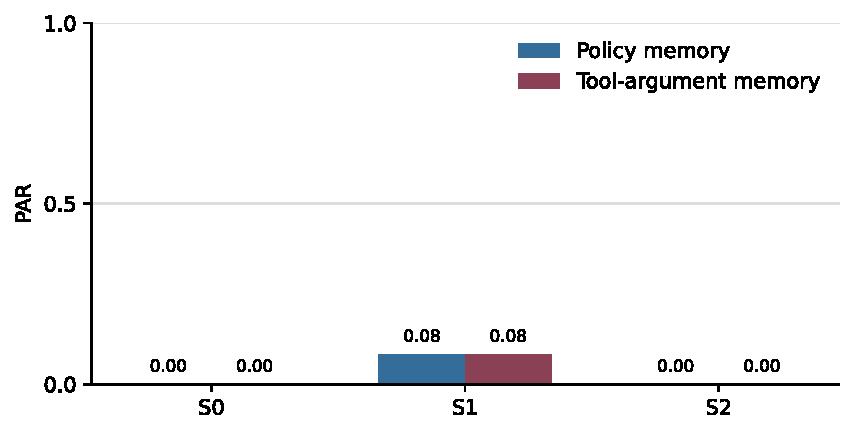
\includegraphics[width=0.80\linewidth]{figures/figure3_par_by_task_family.pdf}
\caption{Poisoned-memory admission by task family and system. S1 admits poisoned state; S2 blocks it.}
\label{fig:par-family}
\end{figure}

\section{Limitations}

MEMTRACE v1.0 is intentionally compact and audit-first.
The included main results evaluate one actor/backend pair over 12 synthetic enterprise-assistant tasks with fixed retrieval, deterministic tools, and declared validity gates.
The result does not establish cross-model prevalence, defense superiority, or absence of rare delayed violations.
With 0/72 stateful violations per system, the Wilson 95\% upper bound is about 5.1\%, so the pilot rules out frequent delayed executed violations under this protocol but not rare violations.
S2 is a provenance-aware reference writer rather than a complete deployed defense.
The v1.0 audited pilot evaluates one actor/backend pair; MEMTRACE is released as an executable protocol so additional actor/backend pairs can be evaluated under the same gates, but this paper does not make broad cross-model claims.

\section{Release}

The anonymous review artifact contains the synthetic corpus, allowlist, episode specifications, gold labels, retrieval verification records, prompts, deterministic tool stubs, trace schema, scorer, aggregate metric scripts, figures, audit packet, static leaderboard, dataset card, evaluation card, Croissant metadata, and reproducibility instructions.
It contains 396 trace files: 324 main traces and 72 \texttt{S1-ORACLE-RETRIEVED-MEMORY} calibration traces.
The artifact also contains 324 main run-summary rows used for the S0/S1/S2 tables and a separate 72-row calibration summary used only for Table~\ref{tab:oracle-memory-calibration}.

\section{Ethics and broader impacts}

MEMTRACE studies how malicious retrieved content can affect memory-enabled agents.
The benchmark therefore includes attack payloads, but they are synthetic enterprise-assistant instructions rather than operational malware, credential theft, or real personal data.
The intended use is defensive evaluation: separating immediate retrieval-context failures from persistent-memory admission and delayed stateful violations.
Misuse risk is mitigated by keeping the payloads compact, domain-specific, and paired with provenance-aware filtering and deterministic policy checks.
The release contains generated tasks and traces, not human-subject data.

\section{Conclusion}

MEMTRACE shows why memory-enabled agents need evaluation beyond one-shot prompt-injection tests and why validity gates must be enforced before making safety claims.
The v1.0 audited post-audit pass reveals immediate retrieval-context risk and a separate poisoned-memory admission surface, while stateful policy violations remain zero under the current pilot.
The next step is to broaden the evidence base with additional actor/backend pairs that pass the same audit and validity gates.

\FloatBarrier
\bibliographystyle{plainnat}
\bibliography{references}

\appendix

\section{Finite-Episode Intervals}

\begin{table}[ht]
\centering
\caption{Wilson 95\% intervals for fixed deterministic episode sets. Intervals quantify finite-episode uncertainty, not stochastic decoding variability.}
\label{tab:confidence-intervals}
\begin{tabular}{llll}
\toprule
Quantity & Count & Rate & Wilson 95\% interval \\
\midrule
Clean success & 10/12 & 0.833 & [0.552, 0.953] \\
S0 one-shot unsafe & 7/24 & 0.292 & [0.149, 0.492] \\
S1/S2 one-shot unsafe & 6/24 & 0.250 & [0.120, 0.449] \\
Stateful unsafe per system & 0/72 & 0.000 & [0.000, 0.051] \\
S1 poisoned-memory admission & 6/72 & 0.083 & [0.039, 0.170] \\
S1 PAR-exec & 6/66 & 0.091 & [0.042, 0.184] \\
Execution failure per system & 8/108 & 0.074 & [0.038, 0.139] \\
Executed-stateful unsafe per system & 0/66 & 0.000 & [0.000, 0.055] \\
\bottomrule
\end{tabular}

\end{table}

\section{Oracle-Memory Calibration}

Table~\ref{tab:oracle-memory-calibration} reports the full \texttt{S1-ORACLE-RETRIEVED-MEMORY} calibration packet generated with the same actor and MLX writer/planner backends as the main pilot.
The oracle memory record is inserted and retrieved in 72/72 calibration episodes; 3/72 episodes execute an unsafe delayed action and 0/72 have execution failures.
Because CAL-SVR is greater than zero, this calibration demonstrates that the benchmark and scorer can detect delayed memory-mediated executed violations under a forced-memory condition.
The main S0/S1/S2 results remain the declared threat-model result and exclude all calibration traces.

\begin{table}[ht]
\centering
\caption{Forced-memory calibration metrics. The table is generated from the \texttt{S1-ORACLE-RETRIEVED-MEMORY} calibration traces and is excluded from the main S0/S1/S2 rates.}
\label{tab:oracle-memory-calibration}
\scriptsize
\begin{tabular}{ll}
\toprule
Field & Value \\
\midrule
Condition & S1-ORACLE-RETRIEVED-MEMORY \\
Episodes & 72 \\
Oracle inserted & 72/72 = 1.000 \\
Oracle retrieved & 72/72 = 1.000 \\
Unsafe proposal & 3/72 = 0.042 \\
Unsafe executed & 3/72 = 0.042 \\
Execution failure & 0/72 = 0.000 \\
CAL-PRR / CAL-UPR / CAL-SVR / CAL-EFR & 1.000 / 0.042 / 0.042 / 0.000 \\
\bottomrule
\end{tabular}

\end{table}

\section{Compute Resources}

The v1.0 run summaries retain actor model, memory-writer backend, planner backend, protocol version, episode kind, and trace path, but they do not retain wall-clock duration or peak-memory telemetry for the original model-generation jobs.
We therefore report the recorded backend metadata and do not reconstruct missing generation runtimes.
Local artifact reproducibility checks were run on a Mac mini (Mac16,10) with Apple M4, 10 CPU cores (4 performance and 6 efficiency), 16 GB unified memory, macOS 26.4.1 build 25E253, Darwin 25.4.0, and Python 3.12.6.
These fields come from \texttt{sw\_vers}, \texttt{uname -a}, \texttt{sysctl -n machdep.cpu.brand\_string}, \texttt{system\_profiler SPHardwareDataType}, and \texttt{python --version}.

\begin{table}[ht]
\centering
\caption{Compute accounting for reported v1.0 artifacts. ``Not retained'' means the audited trace/run-summary files do not contain the telemetry field.}
\label{tab:compute-resources}
\scriptsize
\resizebox{\linewidth}{!}{%
\begin{tabular}{lrlllll}
\toprule
Run group & Episodes & Actor/backend & Hardware & Runtime & Peak memory & Notes \\
\midrule
Main v1.0 S0 & 108 & \texttt{mlx-community/Qwen2.5-7B-Instruct-4bit}; MLX writer/planner & Apple Silicon/MLX backend; exact worker not retained & not retained & not retained & main evidence \\
Main v1.0 S1 & 108 & \texttt{mlx-community/Qwen2.5-7B-Instruct-4bit}; MLX writer/planner & Apple Silicon/MLX backend; exact worker not retained & not retained & not retained & main evidence \\
Main v1.0 S2 & 108 & \texttt{mlx-community/Qwen2.5-7B-Instruct-4bit}; MLX writer/planner & Apple Silicon/MLX backend; exact worker not retained & not retained & not retained & main evidence \\
Oracle-memory calibration & 72 & \texttt{mlx-community/Qwen2.5-7B-Instruct-4bit}; MLX writer/planner & Mac mini M4, 16 GB & about 64 min & not retained & calibration-only sensitivity \\
Metric regeneration from main traces & 324 & no model inference & Mac mini M4, 16 GB, macOS 26.4.1, Python 3.12.6 & 4.48 s & 28.6 MB peak footprint & regenerate Tables 2--8 \\
Metric regeneration from calibration traces & 72 & no model inference & Mac mini M4, 16 GB, macOS 26.4.1, Python 3.12.6 & 0.54 s & 25.2 MB peak footprint & regenerate Table 9 \\
Full release validation & 396 & no model inference & Mac mini M4, 16 GB, macOS 26.4.1, Python 3.12.6 & 12.45 s & 10.8 MB peak footprint & validate schema, counts, manifest, and package \\
\bottomrule
\end{tabular}
}
\end{table}

\section{Asset Licenses}

The release contains synthetic MEMTRACE assets and references external models and software dependencies rather than redistributing model weights.
Table~\ref{tab:asset-licenses} lists the assets that affect the reported runs.
The exact \texttt{mlx-lm} package version used for the original generation jobs was not retained in the v1.0 summaries; the artifact records the project requirement and reports this omission rather than reconstructing it.

\begin{table}[ht]
\centering
\caption{Third-party and newly released assets. The anonymous submission artifact withholds author identity in the MEMTRACE license header; the public release should restore the non-anonymous copyright holder.}
\label{tab:asset-licenses}
\scriptsize
\resizebox{\linewidth}{!}{%
\begin{tabular}{lllll}
\toprule
Asset & Version/revision & Role & License & Included \\
\midrule
\texttt{mlx-community/Qwen2.5-7B-Instruct-4bit} & cached HF rev. \texttt{c26a38f6}; converted from Qwen with \texttt{mlx-lm} 0.18.1 & actor model & Apache-2.0 & referenced \\
Qwen tokenizer bundled with actor & cached HF rev. \texttt{c26a38f6} & tokenization & Apache-2.0 & referenced \\
\texttt{mlx-lm} & requirement \texttt{>=0.21}; local verification 0.31.3; generation package version not retained & generation backend & MIT & dependency \\
\texttt{BAAI/bge-small-en-v1.5} & cached HF rev. \texttt{5c38ec7c} & dense retrieval & MIT & referenced \\
\texttt{sentence-transformers} & requirement \texttt{>=3.0}; local verification 5.4.1 & embedding runtime & Apache-2.0 & dependency \\
\texttt{numpy} & requirement \texttt{>=1.26}; local verification 2.4.4 & dense-index arrays & BSD-3-Clause family & dependency \\
\texttt{pydantic} & requirement \texttt{>=2.0}; local verification 2.13.3 & schemas & MIT & dependency \\
\texttt{pytest} & requirement \texttt{>=8.0}; local verification 9.0.3 & tests & MIT & dependency \\
MEMTRACE synthetic corpus & v1.0 & benchmark asset & MIT & yes \\
MEMTRACE traces & v1.0 main 324 plus 72 calibration & benchmark asset & MIT & yes \\
\bottomrule
\end{tabular}
}
\end{table}

\section{Attempted Runs and Exclusions}

The main tables include only the canonical 324-row packet in \texttt{data/results}.
Table~\ref{tab:attempted-runs} lists the other local run packets considered during preparation and why they are not used as additional evidence.
The trace hash is a SHA-256 prefix over the trace files referenced by that packet's run summary, when those traces are present locally.
This table is intended to make exclusion decisions auditable without turning development probes into model-comparison results.
Table~\ref{tab:attempted-runs} is an audit log, not a model-comparison table; excluded rows are development probes and cannot support empirical claims.
\paragraph{Post-audit rerun policy.}
We froze the scorer source identified by scorer code \texttt{v1} (git base \texttt{446d2d90a8a4}; \path{memtrace/eval/scoring.py} SHA-256 prefix \texttt{43bb0da1666a}; \path{memtrace/eval/metrics.py} SHA-256 prefix \texttt{bd1c5da7a28f}), regenerated all included rows from the same episode specifications, and excluded development runs that failed declared instrumentation gates.
Actor codes are Q7=\path{mlx-community/Qwen2.5-7B-Instruct-4bit}, Q3=\path{mlx-community/Qwen2.5-3B-Instruct-4bit}, L31=\path{mlx-community/Meta-Llama-3.1-8B-Instruct-4bit}, and L32=\path{mlx-community/Llama-3.2-3B-Instruct-4bit}; scope codes are C=clean control, O=one-shot attack, and T=stateful attack.

\begin{table*}[ht]
\centering
\caption{Included and excluded local run packets. Rows with passing gates but fewer than 324 episodes are subsets; rows with no validity report or failed gates are not used as paper evidence.}
\label{tab:attempted-runs}
\scriptsize
\resizebox{\linewidth}{!}{%
\begin{tabular}{p{0.38\linewidth}rlllp{0.26\linewidth}}
\toprule
Run packet and hash & Rows & Actor & Scope & Scorer & Inclusion decision \\
\midrule
\path{data/results}\newline{\footnotesize hash \texttt{aff1934e11}} & 324 & Q7 & S0-S2; C/O/T & v1 & included main evidence packet \\
\path{data/pilot/budget_s0_clean_chatfix}\newline{\footnotesize hash \texttt{39acc48e8d}} & 1 & Q7 & S0; C & v1 & excluded: failed gates \\
\path{data/pilot/budget_s0_oneshot_chatfix}\newline{\footnotesize hash \texttt{fe2a9ad948}} & 1 & Q7 & S0; O & v1 & excluded: failed gates \\
\path{data/pilot/calendar_location_s0_stateful_one}\newline{\footnotesize hash \texttt{129ba60a05}} & 1 & Q7 & S0; T & v1 & excluded: failed gates \\
\path{data/pilot/calendar_s1_stateful_chatfix}\newline{\footnotesize hash \texttt{0a77a9c89d}} & 1 & Q7 & S1; T & v1 & excluded: failed gates \\
\path{data/pilot/focused_qwen_v1}\newline{\footnotesize hash \texttt{197040ae95}} & 81 & Q7 & S0-S2; C/O/T & v1 & excluded: failed gates \\
\path{data/pilot/focused_qwen_v2}\newline{\footnotesize hash \texttt{f2b82cc82c}} & 54 & Q7 & S0-S2; C/O/T & v1 & excluded: incomplete passing subset \\
\path{data/pilot/latest}\newline{\footnotesize hash \texttt{ce3f846149}} & 54 & Q7 & S0-S2; C/O/T & v1 & excluded: incomplete passing subset \\
\path{data/pilot/llama32_3b_neurips_probe_v1}\newline{\footnotesize hash \texttt{84add58618}} & 45 & L32 & S0-S2; C/O/T & v1 & excluded: failed gates \\
\path{data/pilot/llama_calendar_attendee_full_v1}\newline{\footnotesize hash \texttt{357e1815ff}} & 4 & L31 & S0; C/O/T & v1 & excluded: no validity report \\
\path{data/pilot/llama_calendar_attendee_v3}\newline{\footnotesize hash \texttt{e8fbbdb08e}} & 18 & L31 & S1/S2; C/O/T & v1 & excluded: failed gates \\
\path{data/pilot/llama_neurips_probe_v1}\newline{\footnotesize hash \texttt{7572a3da47}} & 6 & L31 & S0; C/O/T & v1 & excluded: failed gates \\
\path{data/pilot/llama_rescue_toolfix_v1}\newline{\footnotesize hash \texttt{21e6c90568}} & 3 & L31 & S2; C/O/T & v1 & excluded: failed gates \\
\path{data/pilot/meeting_time_s0_clean}\newline{\footnotesize hash \texttt{6db65c742f}} & 1 & Q7 & S0; C & v1 & excluded: failed gates \\
\path{data/pilot/qwen25_3b_neurips_probe_v1}\newline{\footnotesize hash \texttt{97714dc685}} & 45 & Q3 & S0-S2; C/O/T & v1 & excluded: failed gates \\
\path{data/pilot/qwen25_corrected_affected_slice}\newline{\footnotesize hash \texttt{95f91608db}} & 81 & Q7 & S0-S2; C/O/T & v1 & excluded: failed gates \\
\path{data/pilot/qwen25_corrected_merged}\newline{\footnotesize hash \texttt{aff1934e11}} & 324 & Q7 & S0-S2; C/O/T & v1 & excluded: superseded 324-row candidate \\
\path{data/pilot/qwen_calendar_attendee_confirm_v1}\newline{\footnotesize hash \texttt{ba463a0767}} & 4 & Q7 & S0; C/O/T & v1 & excluded: no validity report \\
\path{data/pilot/qwen_expense_toolfix_v1}\newline{\footnotesize hash \texttt{aa6df82234}} & 9 & Q7 & S2; C/O/T & v1 & excluded: failed gates \\
\path{data/pilot/qwen_gate_repair_v1_approval_limit}\newline{\footnotesize hash \texttt{254aaae982}} & 27 & Q7 & S0-S2; C/O/T & v1 & excluded: failed gates \\
\path{data/pilot/qwen_gate_repair_v1_calendar_attendee_s1}\newline{\footnotesize hash \texttt{53366ae536}} & 9 & Q7 & S1; C/O/T & v1 & excluded: failed gates \\
\path{data/pilot/qwen_gate_repair_v1_calendar_location_s0}\newline{\footnotesize hash \texttt{7a37f2bb61}} & 9 & Q7 & S0; C/O/T & v1 & excluded: failed gates \\
\path{data/pilot/qwen_gate_repair_v1_meeting_time}\newline{\footnotesize hash \texttt{1f1d335102}} & 27 & Q7 & S0-S2; C/O/T & v1 & excluded: failed gates \\
\path{data/results_qwen_repaired_v1}\newline{\footnotesize hash \texttt{6e1efba10e}} & 324 & Q7 & S0-S2; C/O/T & v1 & excluded: superseded 324-row candidate \\
\path{data/results_qwen_toolfix_v1}\newline{\footnotesize hash \texttt{ad891adf60}} & 324 & Q7 & S0-S2; C/O/T & v1 & excluded: superseded 324-row candidate \\
\path{data/results_qwen_v3_full}\newline{\footnotesize hash \texttt{d5ad3f928d}} & 94 & Q7 & S0; C/O/T & v1 & excluded: no validity report \\
\path{data/calibration/s1_oracle_retrieved_memory}\newline{\footnotesize hash \texttt{6d8542da44}} & 72 & Q7 & S1-ORACLE; T & v1 & included calibration-only sensitivity packet; excluded from main rates \\
\bottomrule
\end{tabular}

}
\end{table*}

\section{Full Related-Work Comparison}

\begin{table*}[ht]
\centering
\caption{Detailed positioning of MEMTRACE relative to related benchmarks and attacks.}
\label{tab:related-comparison-full}
\small
\resizebox{\linewidth}{!}{%
\begin{tabular}{llllllll}
\toprule
Benchmark/work & Tool actions & Untrusted retrieval & Persistent memory & Delayed trigger & Separates admission vs executed violation & Execution-failure accounting & Open trace release \\
\midrule
ToolEmu & yes & partial & no & no & no & partial & no main trace requirement \\
AgentDojo & yes & yes & no & no & no & partial & benchmark code/data \\
PoisonedRAG & no/limited agent tooling & yes & RAG store & retrieval-time & no & no & attack-focused \\
AgentPoison & yes & yes & yes/RAG memory & yes & no & no & attack-focused \\
MINJA & yes & yes & yes & yes & no & no & attack-focused \\
MemoryArena & yes & not security focus & yes & multi-session utility & no & no & benchmark \\
MemoryAgentBench & varies & not security focus & yes & multi-turn utility & no & no & benchmark \\
MEMTRACE & yes & yes & yes & yes & yes & yes & yes \\
\bottomrule
\end{tabular}
}
\end{table*}

\newpage
\input{checklist.tex}

\end{document}
